\documentclass[12pt,a4paper]{article}
\usepackage[UTF8]{ctex}
\usepackage{graphicx,geometry,ulem,enumitem,titlesec,multicol}
\usepackage[export]{adjustbox}
\usepackage{amsmath,amssymb}
\usepackage{fancyhdr,lastpage,tabularx,booktabs,float,subfig}
\usepackage[labelfont=bf]{caption}

% ======= 页眉页脚 =======
\pagestyle{fancy}\fancyhf{}
\fancyhead[C]{\makebox[4.5em][c]{实验名称：}\uline{\makebox[14em][c]{中英双语语音命令实时识别}}\makebox[2.5em][c]{姓名：}\uline{\makebox[4em][c]{巩子杰}}\makebox[2.5em][c]{学号：}\uline{\makebox[5em][c]{3240105977}}}
\fancyfoot[C]{第\thepage 页，共\pageref{LastPage}页}
\renewcommand{\headrulewidth}{0pt}\renewcommand{\footrulewidth}{0pt}
\setlength{\headheight}{50pt}
\fancypagestyle{plain}{\fancyhf{}\renewcommand{\headrulewidth}{0pt}\fancyfoot[C]{第\thepage 页，共\pageref{LastPage}页}}

% ======= 页面 =======
\geometry{left=2.54cm,right=1.5cm,top=2.54cm,bottom=2.54cm}
\renewcommand{\normalsize}{\fontsize{12pt}{18pt}\selectfont}
\titleformat{\section}{\fontsize{16pt}{24pt}\selectfont\bfseries}{\thesection}{1em}{}
\titleformat{\subsection}{\fontsize{15pt}{22.5pt}\selectfont\bfseries}{\thesubsection}{1em}{}
\graphicspath{{../results/v1_english_20/20260611_220716/}{./}}

\begin{document}\thispagestyle{plain}

% ======= 封面 =======
\begin{multicols}{2}
\noindent~\\~\\~\\\hphantom{占位}\raisebox{-0.5\baselineskip}{
\includegraphics[width=1.85in,height=0.58in]{ZJU.jpg}}\hspace{.5em}\raisebox{0pt}[\height][0pt]{\textbf{\fontsize{26pt}{30pt}\selectfont 实验报告}}
\columnbreak
\begin{flushright}
\makebox[3em][l]{专业：}\uline{\makebox[9em][c]{微电子科学与工程}}\\
\makebox[3em][l]{姓名：}\uline{\makebox[9em][c]{巩子杰}}\\
\makebox[3em][l]{学号：}\uline{\makebox[9em][c]{3240105977}}\\
\makebox[3em][l]{日期：}\uline{\makebox[9em][c]{2026年6月10日}}\\
\makebox[3em][l]{地点：}\uline{\makebox[9em][c]{紫金港校区}}\\
\end{flushright}
\end{multicols}
\noindent
课程名称：\uline{信号与系统}\hfill 指导老师：\uline{赵纪伟、郑斌}\hfill 成绩：\uline{\hspace{3cm}}\\
实验名称：\uline{基于梅尔频谱图与CNN的中英双语语音命令实时识别}\hfill 实验类型：\uline{设计类实验}

% ================ 项目背景 ================
\section*{项目背景}

在上一次信号与系统实验课中，我们学习了基于传统信号处理方法的语音识别技术。实验结束后我一直在思考：能否将深度学习引入语音识别中，从而实现更加准确的识别算法？与此同时，在本学期的人工智能课程中，老师详细讲解了卷积神经网络（CNN）用于图像分类的原理，课后的编程作业也涉及 CNN 对图片的视觉分类任务。这让我产生了一个联想：梅尔频谱图本质上是一张二维的"时频图像"——既然 CNN 能够从图片中提取层次化的视觉特征（边缘$\to$纹理$\to$物体局部$\to$整体），那么它同样可以从梅尔频谱图中提取层次化的声学特征（基频$\to$共振峰$\to$音素$\to$词汇）。图像分类和语音命令识别在"二维模式识别"这一点上是相通的，区别只在于输入数据的物理含义不同。

正是这一跨课程的联想，让我我选择了"基于梅尔频谱图与 CNN 的中英双语语音命令实时识别"作为本次课程设计的题目——将信号与系统中的时频分析理论与人工智能课程中的 CNN 分类方法结合起来，探索一条从信号到语义的端到端学习路径。

% ================ 一、实验目的 ================
\section*{一、实验目的}

\begin{enumerate}[leftmargin=*]
\item 掌握语音信号的短时傅里叶变换 (STFT) 与梅尔频谱图的生成方法，理解时频分析的核心地位。
\item 掌握卷积神经网络 (CNN) 在时频特征提取中的应用，理解端到端学习的优势。
\item 通过 \textbf{V1$\to$V2$\to$V3$\to$V4 四个版本迭代}，完整经历从基准建立、多语言扩展、不均衡诊断到数据扩充的科研全流程。
\item 对比 CNN 与 SVM、Random Forest、KNN 等传统方法，验证深度学习的先进性。
\item 验证系统在不同信噪比下的鲁棒性与实时推理的可用性。
\end{enumerate}

\textbf{核心创新点：}将信号与系统的傅里叶变换、滤波器设计等理论与 CNN 端到端学习结合，通过四版本迭代系统性地解决中英双语语音识别中的数据不均衡、跨语言泛化等挑战。

% ================ 二、实验任务与要求 ================
\section*{二、实验任务与要求}

本实验以\textbf{版本迭代}为主线，四个版本逐层递进，每个版本解决前一版本发现的问题：

\begin{table}[H]\centering\caption{四版本迭代任务总览}\label{tab:tasks}
\begin{tabular}{l|c|c|c|l}
\toprule
\textbf{版本} & \textbf{类别} & \textbf{EN:ZH} & \textbf{核心策略} & \textbf{要解决的问题} \\
\midrule
V1 & 20 (纯EN) & — & 标准 CNN + SpecAugment & 基准建立: 方案可行吗? \\
V2 & 40 (中英) & 52:1 & 直接联合训练 & 多语言扩展: 模型容量够吗? \\
V3 & 40 (中英) & 52:1 & \textbf{类别加权损失} & 不均衡: 中文被忽略怎么办? \\
V4 & 40 (中英) & 8.2:1 & \textbf{扩数据} + 弱类别加权 & 扩充: 更多数据 = 更好? \\
\bottomrule
\end{tabular}
\end{table}


% ================ 三、实验原理 ================
\section*{三、实验原理}

\subsection*{3.1 信号处理流水线}

语音在 10--30 ms 内近似平稳。六步流水线将其转化为二维时频表征:

\textbf{(1) 预加重}：$y[n]=x[n]-0.97\cdot x[n-1]$，$H(z)=1-0.97z^{-1}$，一阶高通 FIR 补偿高频衰减。

\textbf{(2) 分帧加窗}：帧长 400 点(25 ms)，帧移 160 点(10 ms)，60\% 重叠。汉明窗 $w[n]=0.54-0.46\cos(2\pi n/(N-1))$，旁瓣衰减 $-43$ dB。

\textbf{(3) STFT}：$X_m[k]=\sum_{n=0}^{N-1}\tilde{x}_m[n]e^{-j2\pi kn/K}$，$K=512$，$P_m[k]=|X_m[k]|^2/K$。

\textbf{(4) Mel 滤波器组}：$f_{\text{mel}}=2595\log_{10}(1+f_{\text{Hz}}/700)$，128 个非均匀三角滤波器，$S_m[b]=\sum_k P_m[k]H_b[k]$。

\textbf{(5) 对数压缩}：$S_m^{\text{dB}}[b]=10\log_{10}(S_m[b]+10^{-6})$，模仿人耳对数感知。

\textbf{(6) Z-score 归一化}：$\hat{S}= (S-\mu)/\sigma$。最终输出 $128\times98$ 梅尔频谱图。

\subsection*{3.2 CNN 架构}

3 个卷积块(32$\to$64$\to$128 通道) + GAP + FC(256$\to$C)。
参数量 $\sim$330K。逐层增加通道数学习层次化特征；GAP 替代 Flatten；Dropout(0.2--0.5) 防过拟合；Kaiming 初始化 + BatchNorm 稳定训练。

\subsection*{3.3 关键策略演进}

\textbf{SpecAugment}（V1--V4 通用）：频率遮盖($\le$27 频带$\times$2) + 时间遮盖($\le$25 帧$\times$2)，迫使模型从部分信息学习完整表示。

\textbf{类别加权}（V3/V4）：V3 使用完整倒频率加权 $w_c=\frac{C/n_c}{\sum_i C/n_i}$；V4 在中文样本扩充后采用较弱的平方根加权 $w_c\propto n_c^{-0.5}$，避免过度补偿少数类。

\textbf{过采样诊断}：曾尝试 WeightedRandomSampler 强制中英采样均衡，但与类别加权叠加后训练不稳定，最终 V4 采用“扩充中文数据 + 弱加权”的方案。

\subsection*{3.4 系统流程图}

\begin{figure}[H]\centering
\fbox{\begin{minipage}{0.92\textwidth}\centering\vspace{4pt}
原始音频 $\to$ 预加重 $\to$ 分帧加窗 $\to$ STFT $\to$ Mel 滤波器组 $\to$ 对数压缩 $\to$ \textbf{梅尔频谱图 (128$\times$98)} $\to$ \textbf{2D CNN (3 Blocks)} $\to$ 分类(40类)
\vspace{4pt}\end{minipage}}
\caption{系统总体流程}\label{fig:flow}
\end{figure}

% ================ 四、实验方案设计 ================
\section*{四、实验方案设计与参数计算}

\subsection*{4.1 信号处理参数}

\begin{table}[H]\centering\caption{信号处理参数与理论依据}
\begin{tabular}{l|c|l}\toprule
\textbf{参数}&\textbf{值}&\textbf{理论依据}\\\midrule
采样率&16 kHz&Nyquist: $f_s\ge2\times8$kHz\\
帧长&25 ms(400点)&短时平稳假设(10--30 ms)\\
帧移&10 ms(160点)&60\%重叠保证连续性\\
窗函数&Hamming&旁瓣衰减$-43$ dB\\
FFT点数&512&2的幂，补零提高密度\\
Mel频带数&128&分辨率与计算量平衡\\\bottomrule
\end{tabular}
\end{table}

\subsection*{4.2 训练超参数}

\begin{table}[H]\centering\caption{训练配置(四版本统一)}
\begin{tabular}{l|l}\toprule
损失函数&交叉熵+标签平滑($\epsilon=0.1$)\\
优化器&AdamW(lr=$10^{-3}$,$\beta_1=0.9$,$\beta_2=0.999$,decay=$10^{-4}$)\\
调度&ReduceLROnPlateau(factor=0.5,patience=8)\\
早停&patience=20, 最大100轮\\\bottomrule
\end{tabular}
\end{table}

\subsection*{4.3 数据集}

\begin{table}[H]\centering\caption{数据集统计(四版本对比)}
\begin{tabular}{l|c|c|c|c}\toprule
&\textbf{V1}&\textbf{V2}&\textbf{V3}&\textbf{V4}\\\midrule
英文样本&77,454&77,454&77,454&77,454\\
中文样本&—&1,497&1,497&\textbf{9,491}\\
EN:ZH&—&52:1&52:1&\textbf{8.2:1}\\
训练集&54,218&55,267&55,267&\textbf{60,863}\\
测试集中文&—&222&222&\textbf{1,462}\\\bottomrule
\end{tabular}
\end{table}

英文数据来自 \textbf{Google Speech Commands v2 (GSC v2)}：Google 发布的开源语音命令数据集，包含来自 2,618 名不同说话人的 105,829 条语音。本实验选用其中 20 类英文命令词（yes, no, up, down, left, right, on, off, stop, go 及 0--9 共十个数字），总计 77,454 条样本，覆盖不同年龄、性别和口音的说话人，提供了丰富的声学多样性。

V4 中文来自 Microsoft Edge TTS: 实际有效声音/语速组合约为 15 组（5 种声音 $\times$ 3 种语速），每类约 475 条。

% ================ 五、实验仪器设备 ================
\section*{五、实验仪器设备}

\begin{table}[H]\centering\caption{软硬件环境}
\begin{tabular}{l|l}\toprule
操作系统&Windows 11\\
CPU/GPU&Intel Core i7 / NVIDIA GeForce RTX\\
Python&3.9+\\
框架&PyTorch 2.0+, librosa, scikit-learn\\
TTS&Microsoft Edge TTS (edge-tts)\\\bottomrule
\end{tabular}
\end{table}

% ================ 六、实验步骤与数据记录 ================
\section*{六、实验步骤、调试过程与数据记录}

\textbf{以 V1$\to$V2$\to$V3$\to$V4 的顺序进行}，完整记录每个版本的实验过程、遇到的问题及解决方案。

\subsection*{6.1 V1: 英文基准}

\textbf{目的}：验证梅尔频谱图 + CNN 方案在语音命令识别上的可行性。

\textbf{过程}：使用 Google Speech Commands v2 (GSC v2) 纯英文 20 类数据，来自 2,618 名说话人的 77,454 条语音，训练 100 轮。数据预处理 $\sim$20 分钟，GPU 训练 $\sim$15 分钟。

\begin{table}[H]\centering\caption{V1 训练记录}\label{tab:v1train}
\begin{tabular}{l|c}\toprule
训练集/验证集/测试集&54,218 / 11,618 / 11,618\\
最佳轮次&Epoch 96/100\\
最佳验证准确率&96.52\%\\\bottomrule
\end{tabular}
\end{table}

训练过程输出示例：

\begin{verbatim}
Epoch [ 96/100] Train Loss: 1.262 | Train Acc: 79.60% |
               Val Loss: 0.867 | Val Acc: 96.52% *

[Checkpoint] Best model saved (acc=96.52%)
Training complete!  Best val acc: 96.52% at epoch 96
  Total time: 14.5 min

============================================================
TEST RESULTS
  Loss:     0.880
  Accuracy: 96.49%
============================================================
\end{verbatim}

\textbf{结论}：方案可行性得到验证，准确率可以达到96.49\% 。

\subsection*{6.2 V2: 中英扩展}

\textbf{目的}：将系统从 20 类英文扩展至 40 类中英双语，验证跨语言能力。

\textbf{过程}：TTS 合成 20 类中文(1,497 条)，与英文混合(52:1)。直接训练 100 轮。

\textbf{踩坑}：首次评估中文全部 Support=0。排查发现 evaluate.py 默认加载 V1 数据目录。修复：读取模型 config.json 的 NUM\_CLASSES 自动匹配数据目录，加载后验证标签一致性。

\subsection*{6.3 V3: 加权平衡}

\textbf{目的}：解决 V2 暴露的 52:1 极度不均衡问题。根因分析：标准 CE 下，模型可通过"永远输出英文"获得 $\sim$98\% 准确率，中文类别的梯度被淹没。

\textbf{方案}：类别加权 $w_c\propto 1/n_c$，中文自动获得 $\sim$50$\times$ 损失权重。

训练启动时输出的类别权重：

\begin{verbatim}
[INFO] Class weights: EN avg=0.2  ZH avg=51.8
Trainer initialized
  Device:      cuda
  Model:       330,184 params
  Optimizer:   AdamW
  Class weight: enabled (ZH weight approx. 50x)

Epoch [ 99/100] Train Loss: 1.185 | Train Acc: 78.39% |
               Val Loss: 0.874 | Val Acc: 95.47% *

Training complete!  Best val acc: 95.47% at epoch 99
============================================================
TEST RESULTS
  Overall: 94.29%  |  EN: 94.5%  |  ZH: 82.9%
============================================================
\end{verbatim}

\subsection*{6.4 V4: 数据扩充}

\textbf{目的}：V3 中文 82.9\% 仍有提升空间。假设：增加中文数据量可进一步提升。

\textbf{方案}：TTS 扩至 9,491 条(8.2:1)，训练时采用平方根类别加权($w_c\propto n_c^{-0.5}$)，不再启用过采样。早期曾尝试“过采样 + 完整倒频率加权”双重补偿，但该组合使验证准确率长期停留在约 15\%，说明少数类补偿过强会破坏整体优化，因此最终改为更保守的弱加权方案。

\textbf{过程}：扩 TTS $\sim$1 小时，预处理 $\sim$25 分钟，GPU 训练 $\sim$20 分钟。

\begin{verbatim}
[INFO] Class weights enabled
[INFO] Class weight power: 0.50
[INFO] Data dir: ../data/processed_mixed_v4

Epoch [ 97/100] ... Val Acc: 94.83% *

Training complete!  Best val acc: 94.83% at epoch 97
============================================================
TEST RESULTS
  Overall: 95.15%  |  EN: 94.54%  |  ZH(TTS): 100.00%
============================================================
\end{verbatim}

\subsection*{6.5 四版本模型总览}

训练完成后，项目自动记录所有版本：

\begin{verbatim}
$ python evaluate.py --list_models

======================================================================
  AVAILABLE MODELS
======================================================================
  [0] v2_bilingual_40/bilingual_v4_weighted_sqrt
      Test Acc: 95.15%  |  Val Acc: 94.83%  <-- LATEST
  [1] v2_bilingual_40/bilingual_v3_weighted
      Test Acc: 94.29%  |  Val Acc: 95.47%
  [2] v2_bilingual_40/bilingual_v1
      Test Acc: 95.46%  |  Val Acc: 95.47%
  [3] v1_english_20/20260611_220716
      Test Acc: 96.49%  |  Val Acc: 96.52%
======================================================================
\end{verbatim}

\subsection*{6.6 泛化能力验证——真人语音交互测试}

测试集评估只能反映模型在"已知数据分布"上的表现。为验证模型的真实泛化能力，开发了交互式语音测试工具 interactive\_test.py，使用真人语音对模型进行盲测。

\textbf{测试流程}：程序在屏幕上依次显示要说的词汇（随机打乱顺序），测试者按 Enter 键后对着麦克风说出该词，系统完成录音、预处理、推理并实时显示 Top-3 预测结果。所有录音自动保存，测试结束后生成 JSON 和 TXT 双格式汇总报告，包含总体准确率、中英文分别统计和每词明细。


\textbf{保存录音测试}：编写 \texttt{evaluate\_recordings.py}，对 \texttt{recordings/} 中已保存的 99 条真人 UI 录音使用当前 V4 模型重新推理，并按文件名解析真实标签。
\begin{center}
\begin{tabular}{lccc}\toprule
\textbf{测试来源} & \textbf{样本数} & \textbf{正确数} & \textbf{准确率}\\\midrule
保存 UI 录音总体 & 99 & 40 & 40.40\%\\
英文 UI 录音 & 61 & 40 & 65.57\%\\
中文 UI 录音 & 38 & 12 & 31.58\%\\\bottomrule
\end{tabular}
\end{center}

可以发现，真实录音测试时的效果比较差，尤其是中文词汇只有31.58\% 。由于该 UI 录音集规模较小、录制条件不完全受控，因此它不能替代正式大规模真人测试；但它足以说明：\textbf{TTS 中文测试集 100\% 不能泛化到到真实中文 UI 输入}。可能原因是：(1) 真人语音存在麦克风频响差异、房间混响、口音、语速、音高和发音强弱变化，这些因素在 TTS 数据中覆盖不足；(2) TTS 语音过于"标准"，不同重复样本之间只有有限变化，模型容易适应合成语音模板；(3) UI 录音时还包含静音截断、说话起止点偏移、环境噪声和录音设备自动增益等额外变量。

\subsection*{6.7 图形化交互测试工具 (GUI)}

为进一步提升测试的易用性和直观性，我基于实验课程中的GUI界面设计，开发了类似的图形化语音识别测试工具 \texttt{gui\_test.py}。

\begin{figure}[H]
\centering
\subfloat[测试内容选择界面]{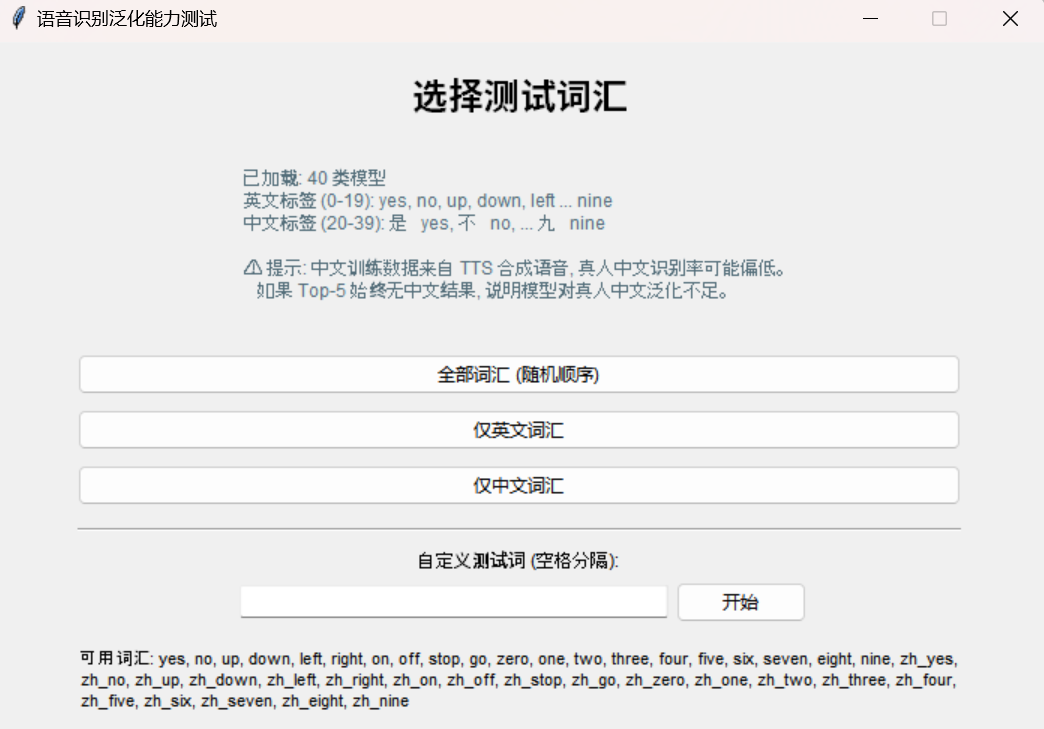
\includegraphics[width=0.48\textwidth]{gui_select.png}}
\subfloat[实时识别界面]{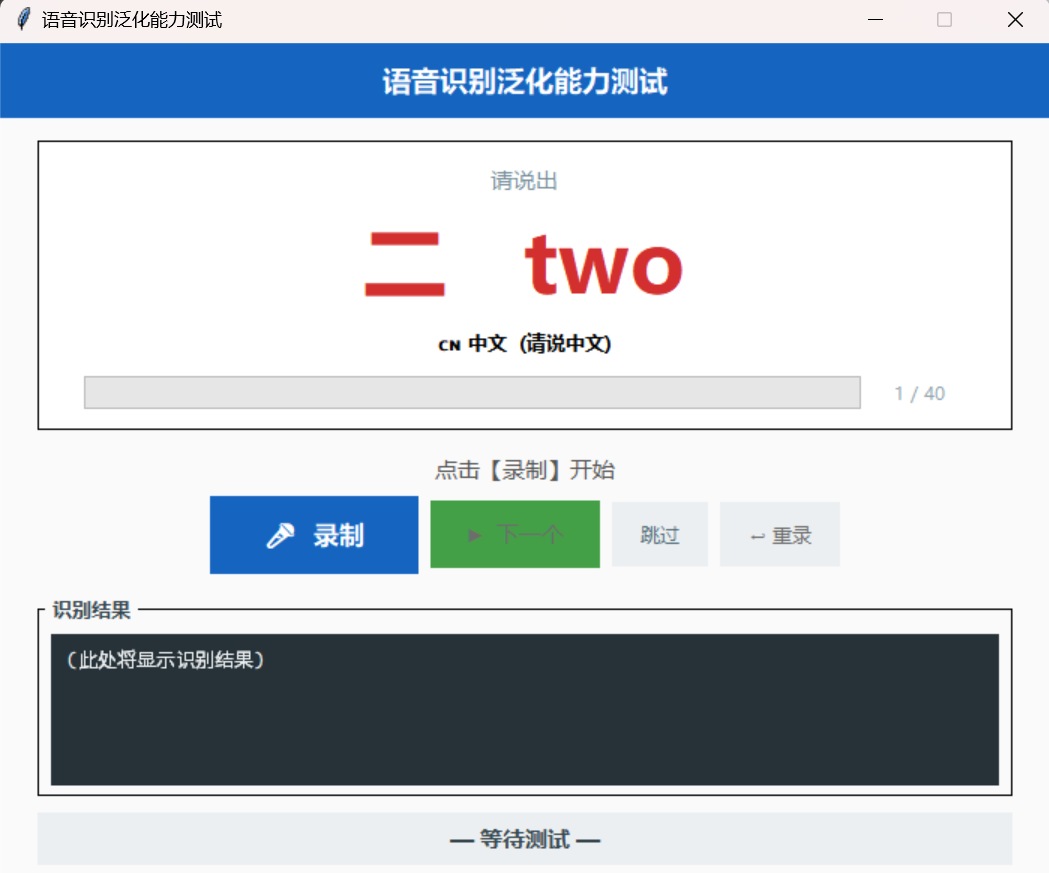
\includegraphics[width=0.48\textwidth]{gui_infer.png}}
\caption{GUI 语音识别测试工具}
\label{fig:gui}
\end{figure}

测试内容选择界面（图 \ref{fig:gui}a）：启动时用户可选择模型版本（V1 / V4 / 自定义），系统自动加载对应模型和词汇表，支持设置每词重复次数和随机打乱顺序。

实时识别界面（图 \ref{fig:gui}b）：点击「开始录音」后录制 1.5 秒语音，自动完成预处理和 CNN 推理。界面实时显示 Top-3 预测及置信度柱状图、当前进度和累计准确率（总体/英文/中文）。测试完成后弹出汇总窗口，显示每类单词的详细准确率，所有结果自动保存。

\subsection*{6.8 实时推理}

inference.py --record 模式：录音 1.5s $\to$ 预处理 $\to$ CNN 推理 $<$5ms(GPU)。

% ================ 七、数据分析 ================
\section*{七、数据分析}

\subsection*{7.1 四版本结果对比}

\begin{table}[H]\centering\caption{V1--V4 完整性能对比(核心表格)}\label{tab:v1v4}
\begin{tabular}{l|c|c|c|c}\toprule
\textbf{指标}&\textbf{V1 英文基准}&\textbf{V2 中英未加权}&\textbf{V3 中英加权}&\textbf{V4 扩充+弱加权}\\\midrule
类别数&20&40&40&40\\
EN:ZH&—&52:1&52:1&\textbf{8.2:1}\\
策略&标准CE&标准CE&\textbf{加权CE}&扩数据+$n_c^{-0.5}$弱加权\\\midrule
\textbf{总体 Acc}&\textbf{96.49\%}&95.46\%&94.29\%&95.15\%\\
\textbf{英文 Acc}&\textbf{96.49\%}&95.8\%&94.5\%&94.54\%\\
\textbf{中文 Acc}&—&76.1\%&\textbf{82.9\%}&\textbf{100.0\% (TTS)}\\
Macro F1&0.965&0.839&0.822&0.973\\
参数量&325K&330K&330K&330K\\\bottomrule
\end{tabular}
\end{table}

\textbf{迭代分析}：

\textbf{V1$\to$V2}：类别翻倍(20$\to$40)，总体仅降 1.03pp，证明 CNN 容量充足。但中文 76.1\% 远低于英文，暴露了 52:1 的致命不均衡。

\textbf{V2$\to$V3}：类别加权使中文提升 6.8pp(76.1\%$\to$82.9\%)！代价是英文降 1.3pp ——典型的精度--公平性权衡。V3 说明在中文数据量不变时，损失函数重加权能有效改善少数类识别。

\textbf{V3$\to$V4}：中文 TTS 数据扩充后，V4 在自动划分的 TTS 中文测试集上达到 100.0\%，总体准确率为 95.15\%。但该结果不能直接解释为“真实中文语音识别 100\%”：它反映的是模型对当前 TTS 数据分布的拟合能力；保存 UI 录音复评中，中文真人录音为 12/38，说明真实 UI 输入仍然明显更困难。

\begin{figure}[H]\centering
\subfloat[训练与验证曲线]{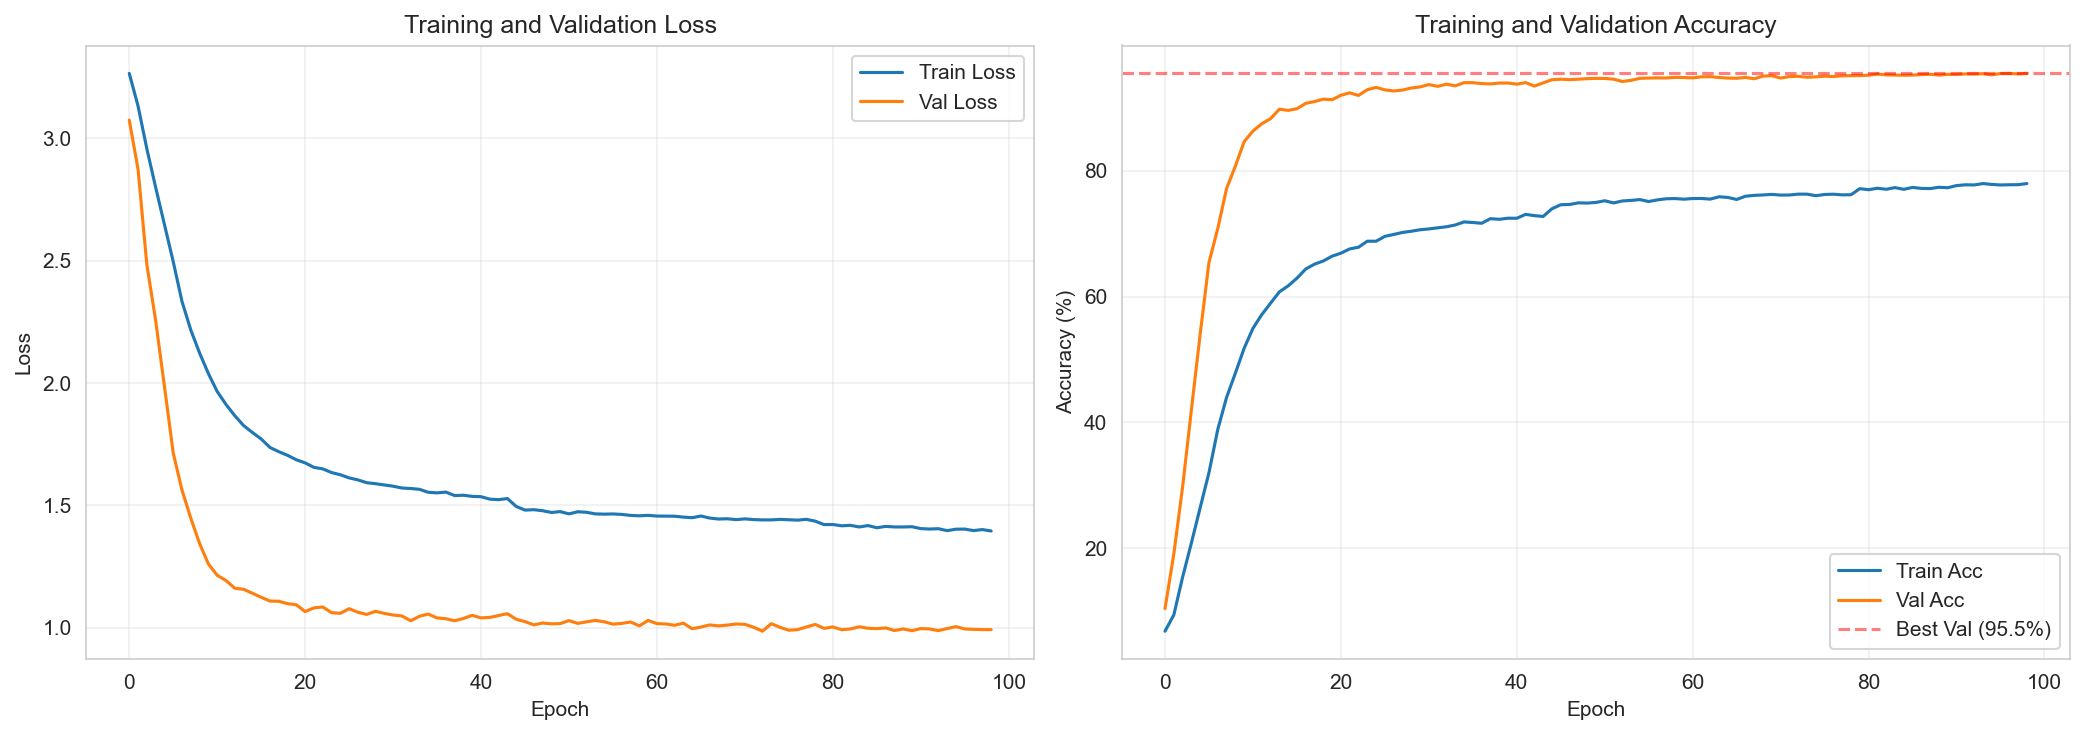
\includegraphics[width=0.32\textwidth]{training_history.png}}
\subfloat[归一化混淆矩阵]{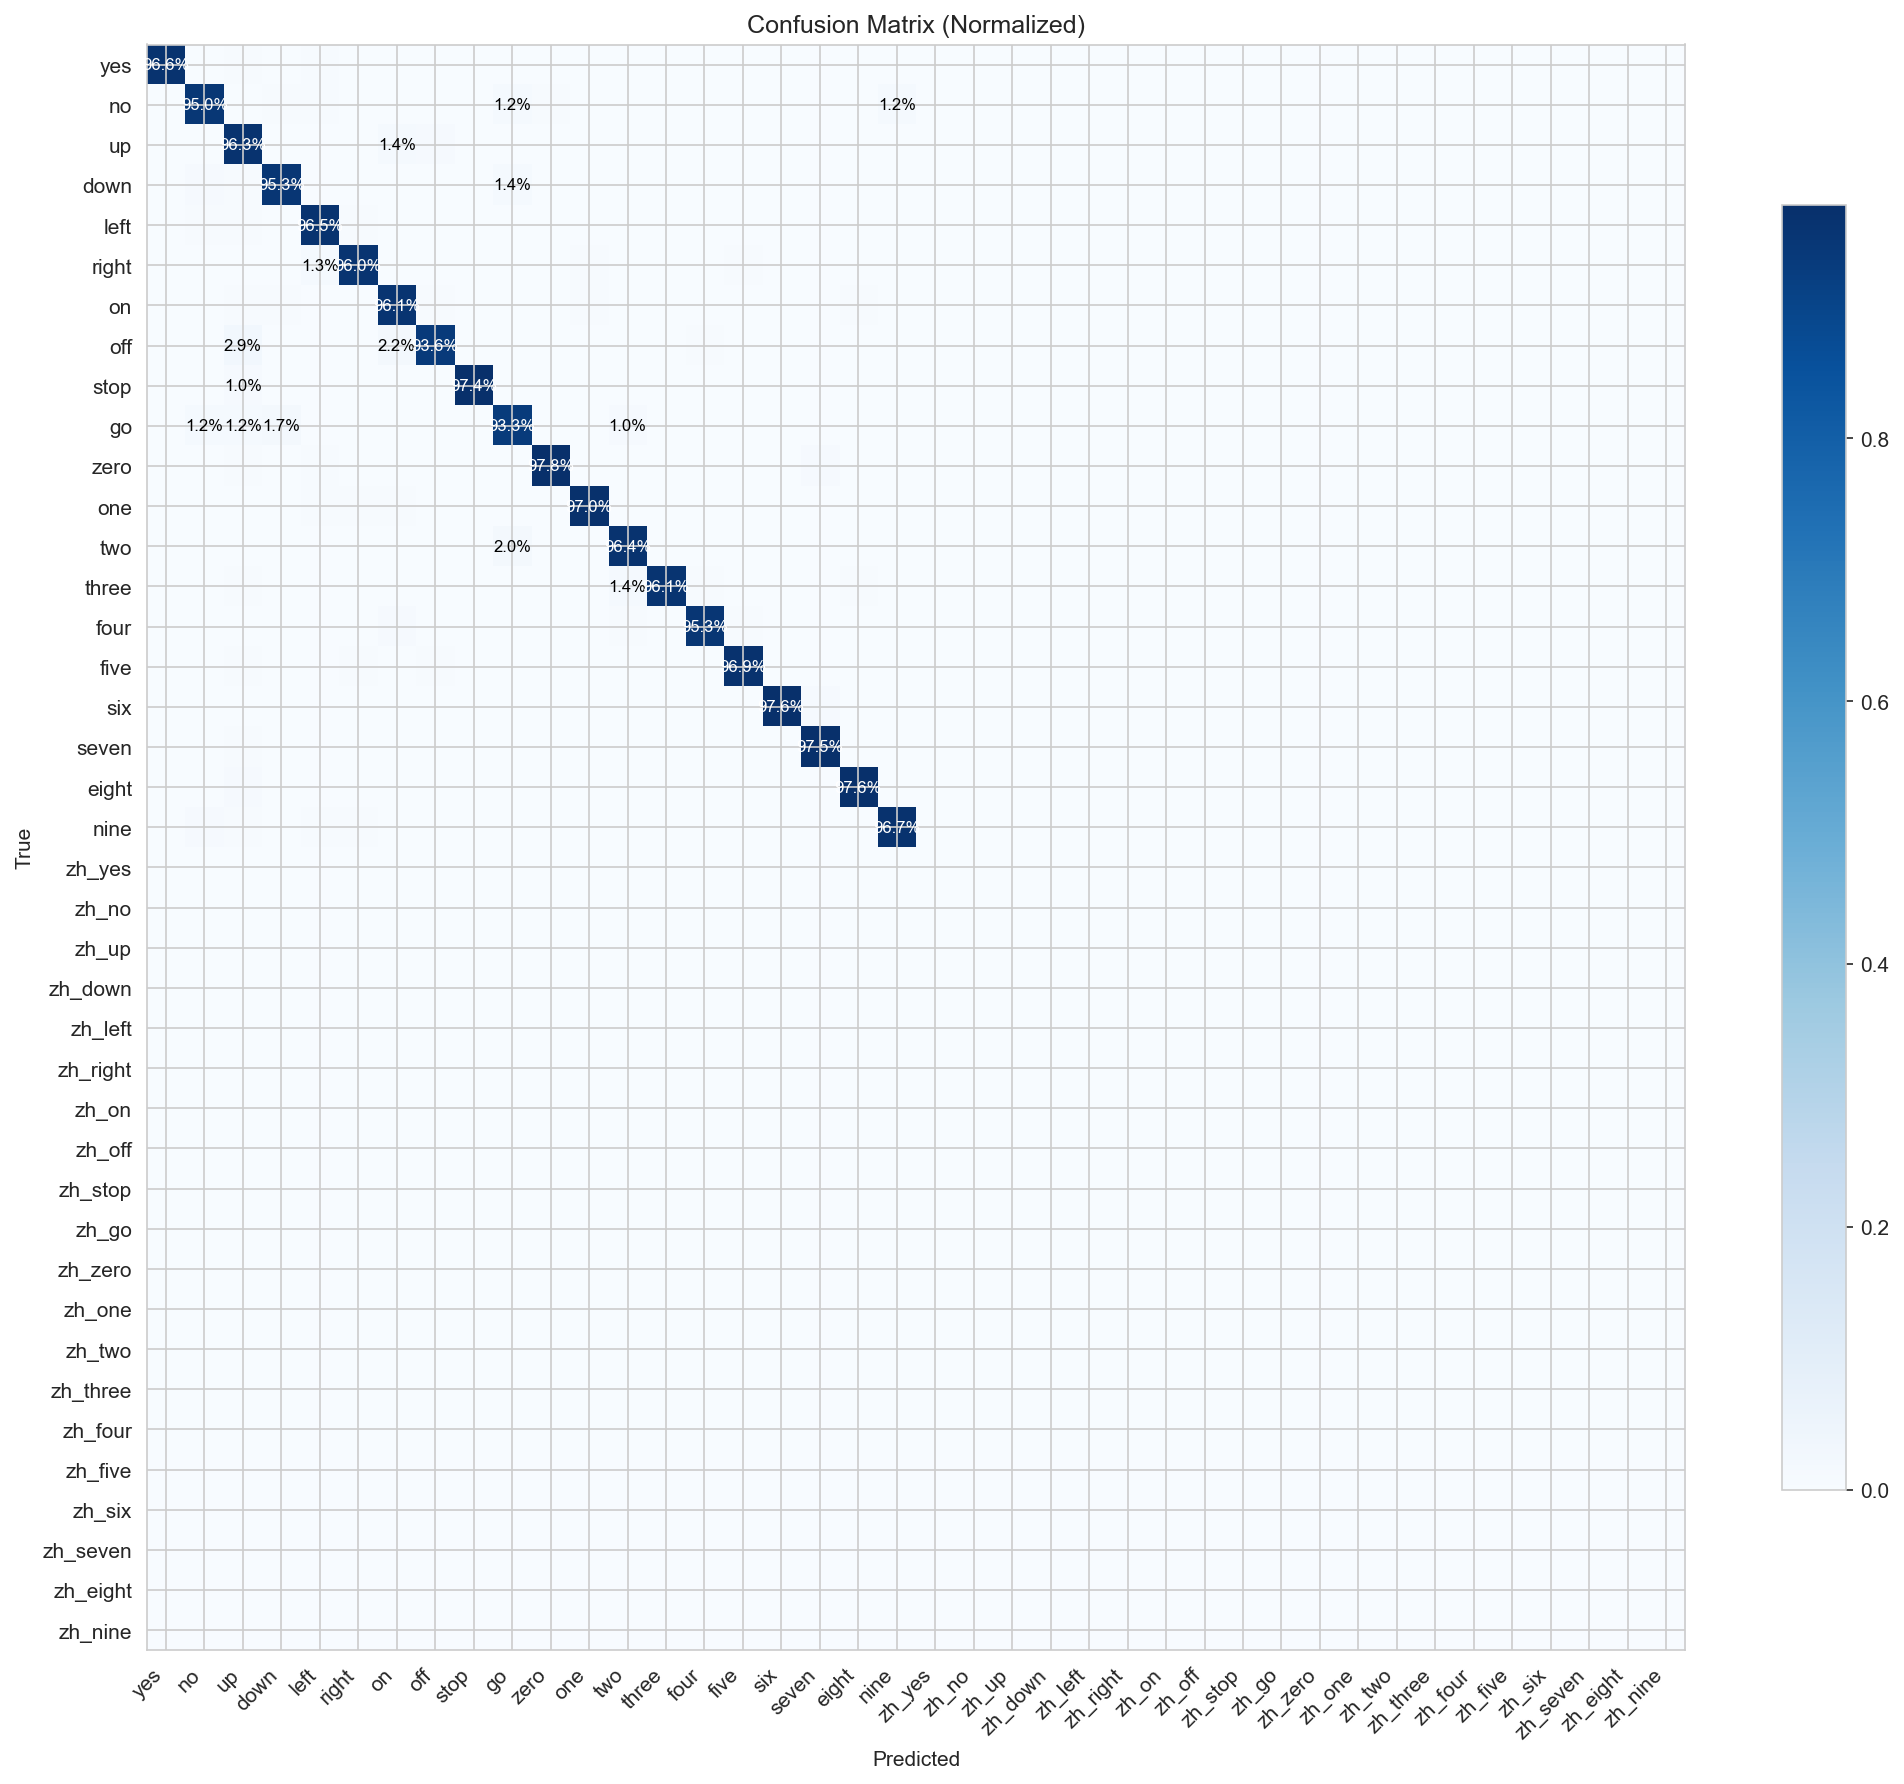
\includegraphics[width=0.32\textwidth]{confusion_matrix_normalized.png}}
\subfloat[ROC 曲线 (one-vs-rest)]{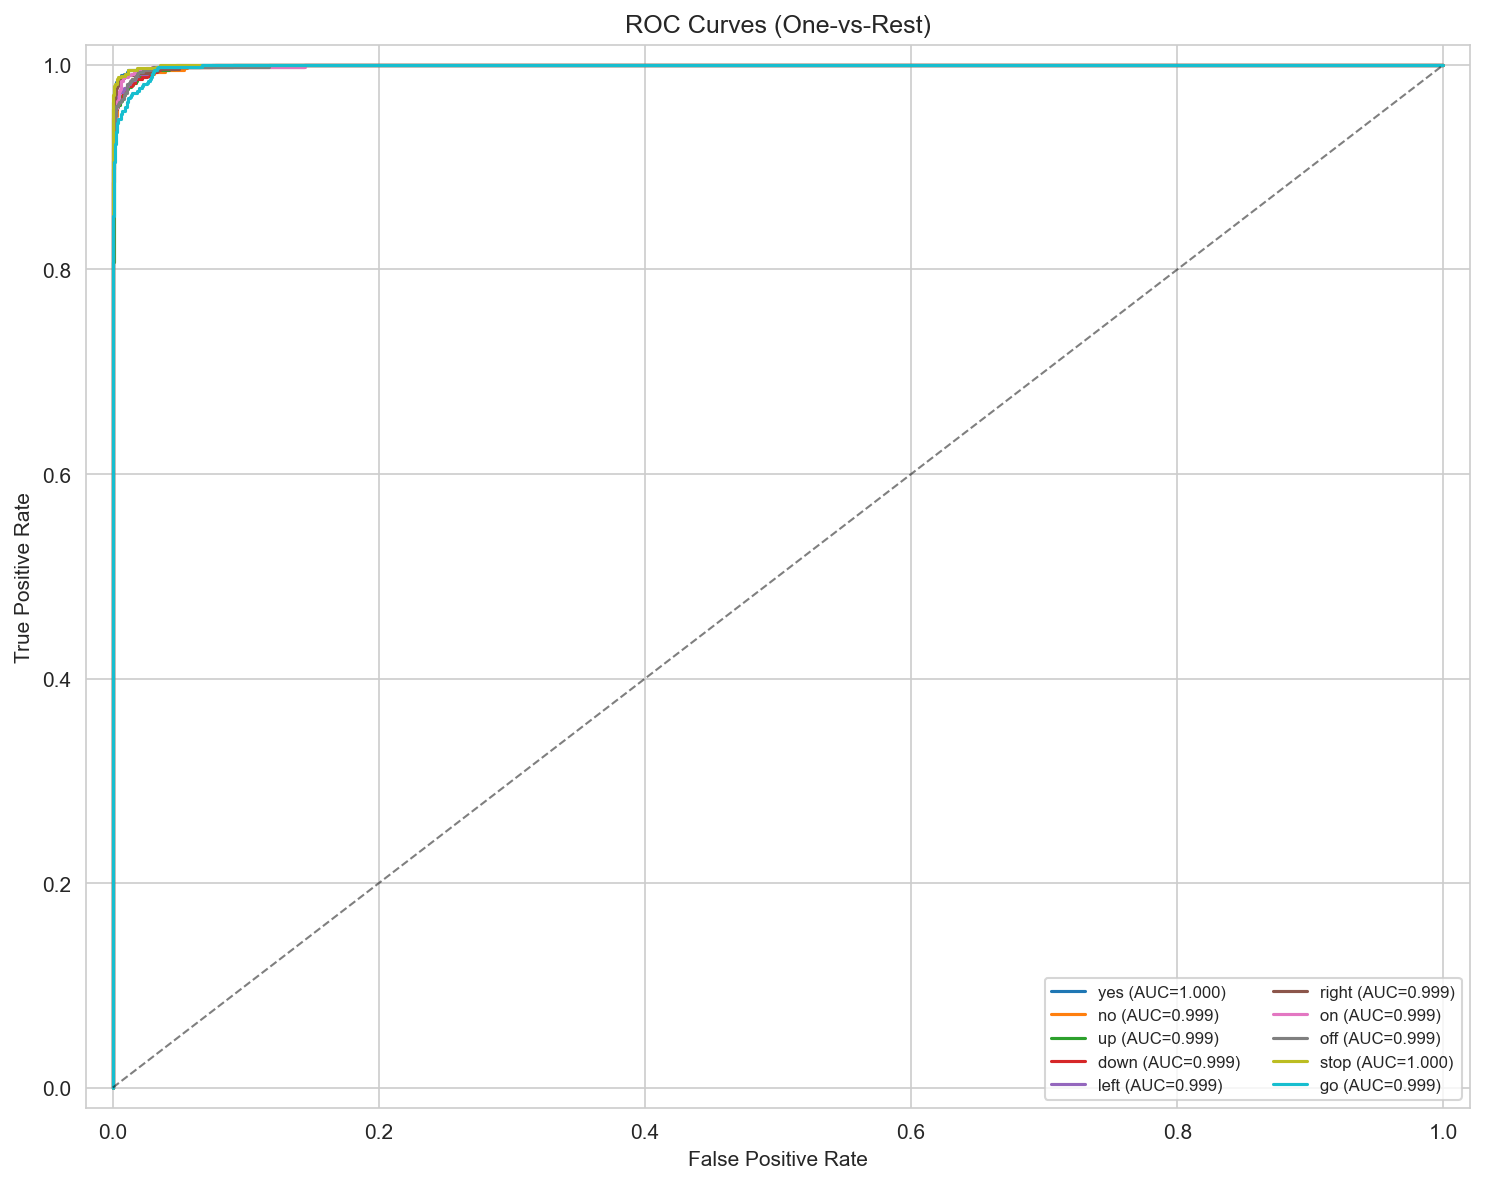
\includegraphics[width=0.32\textwidth]{roc_curves.png}}
\caption{V1 英文 20 类基准——训练过程与评估结果}
\label{fig:v1all}
\end{figure}

图 \ref{fig:v1all}(a) 为 V1 的训练和验证曲线。两条 Loss 曲线均平滑下降且未出现"验证 Loss 上升、训练 Loss 下降"的过拟合特征，训练准确率（终值 79.6\%）始终低于验证准确率（终值 96.5\%），起到了正则化效果。

图 \ref{fig:v1all}(b) 为归一化混淆矩阵（20$\times$20）。对角线从 0.88 到 0.98 不等，颜色明亮且集中，表明模型对各类别均有优秀的区分力。表现最弱的 ``up'' 类（精确率 87.8\%），其非对角线能量主要分散在 ``on'' 和 ``off'' 等短单词上，可能原因有这些词的时频谱结构存在相似性。

图 \ref{fig:v1all}(c) 为各类别的 ROC 曲线。所有 20 条曲线均紧贴左上角，AUC 普遍在 0.995 以上——说明分类器不仅准确率高，而且在不同决策阈值下均保持优异的灵敏度和特异度平衡。

\begin{figure}[H]\centering
\subfloat[V3 归一化混淆矩阵 (40 类)]{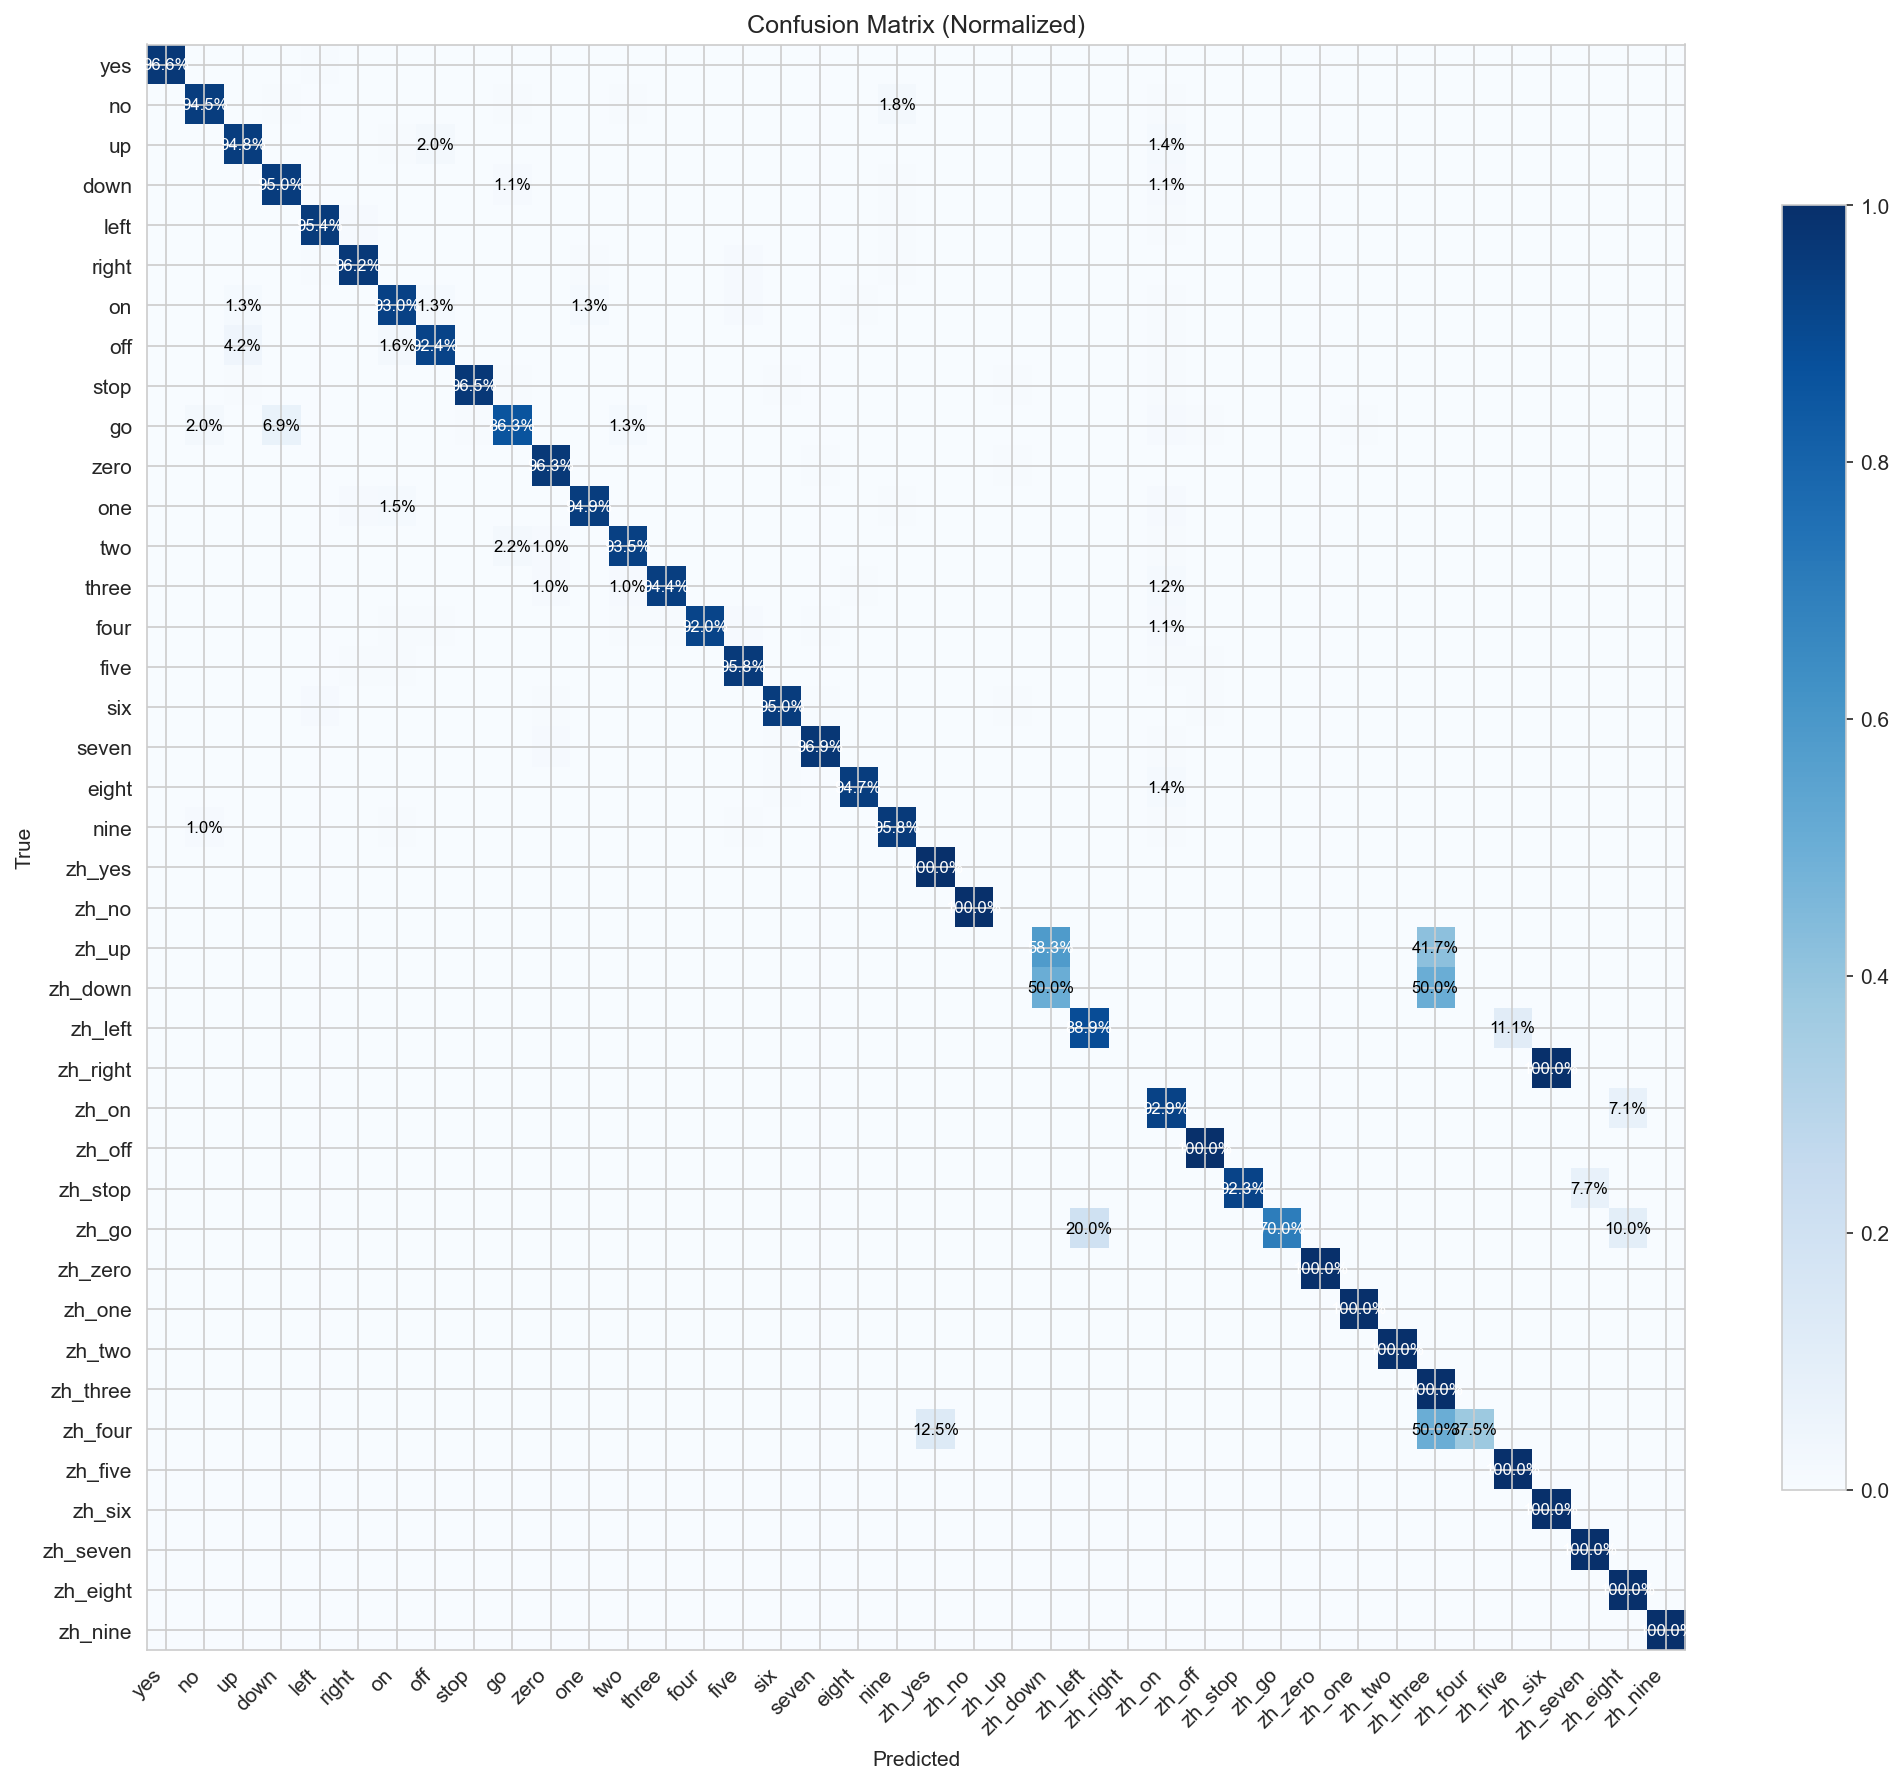
\includegraphics[width=0.48\textwidth]{../results/v2_bilingual_40/bilingual_v3_weighted/confusion_matrix_normalized.png}}
\subfloat[V3 特征空间的 t-SNE 二维投影]{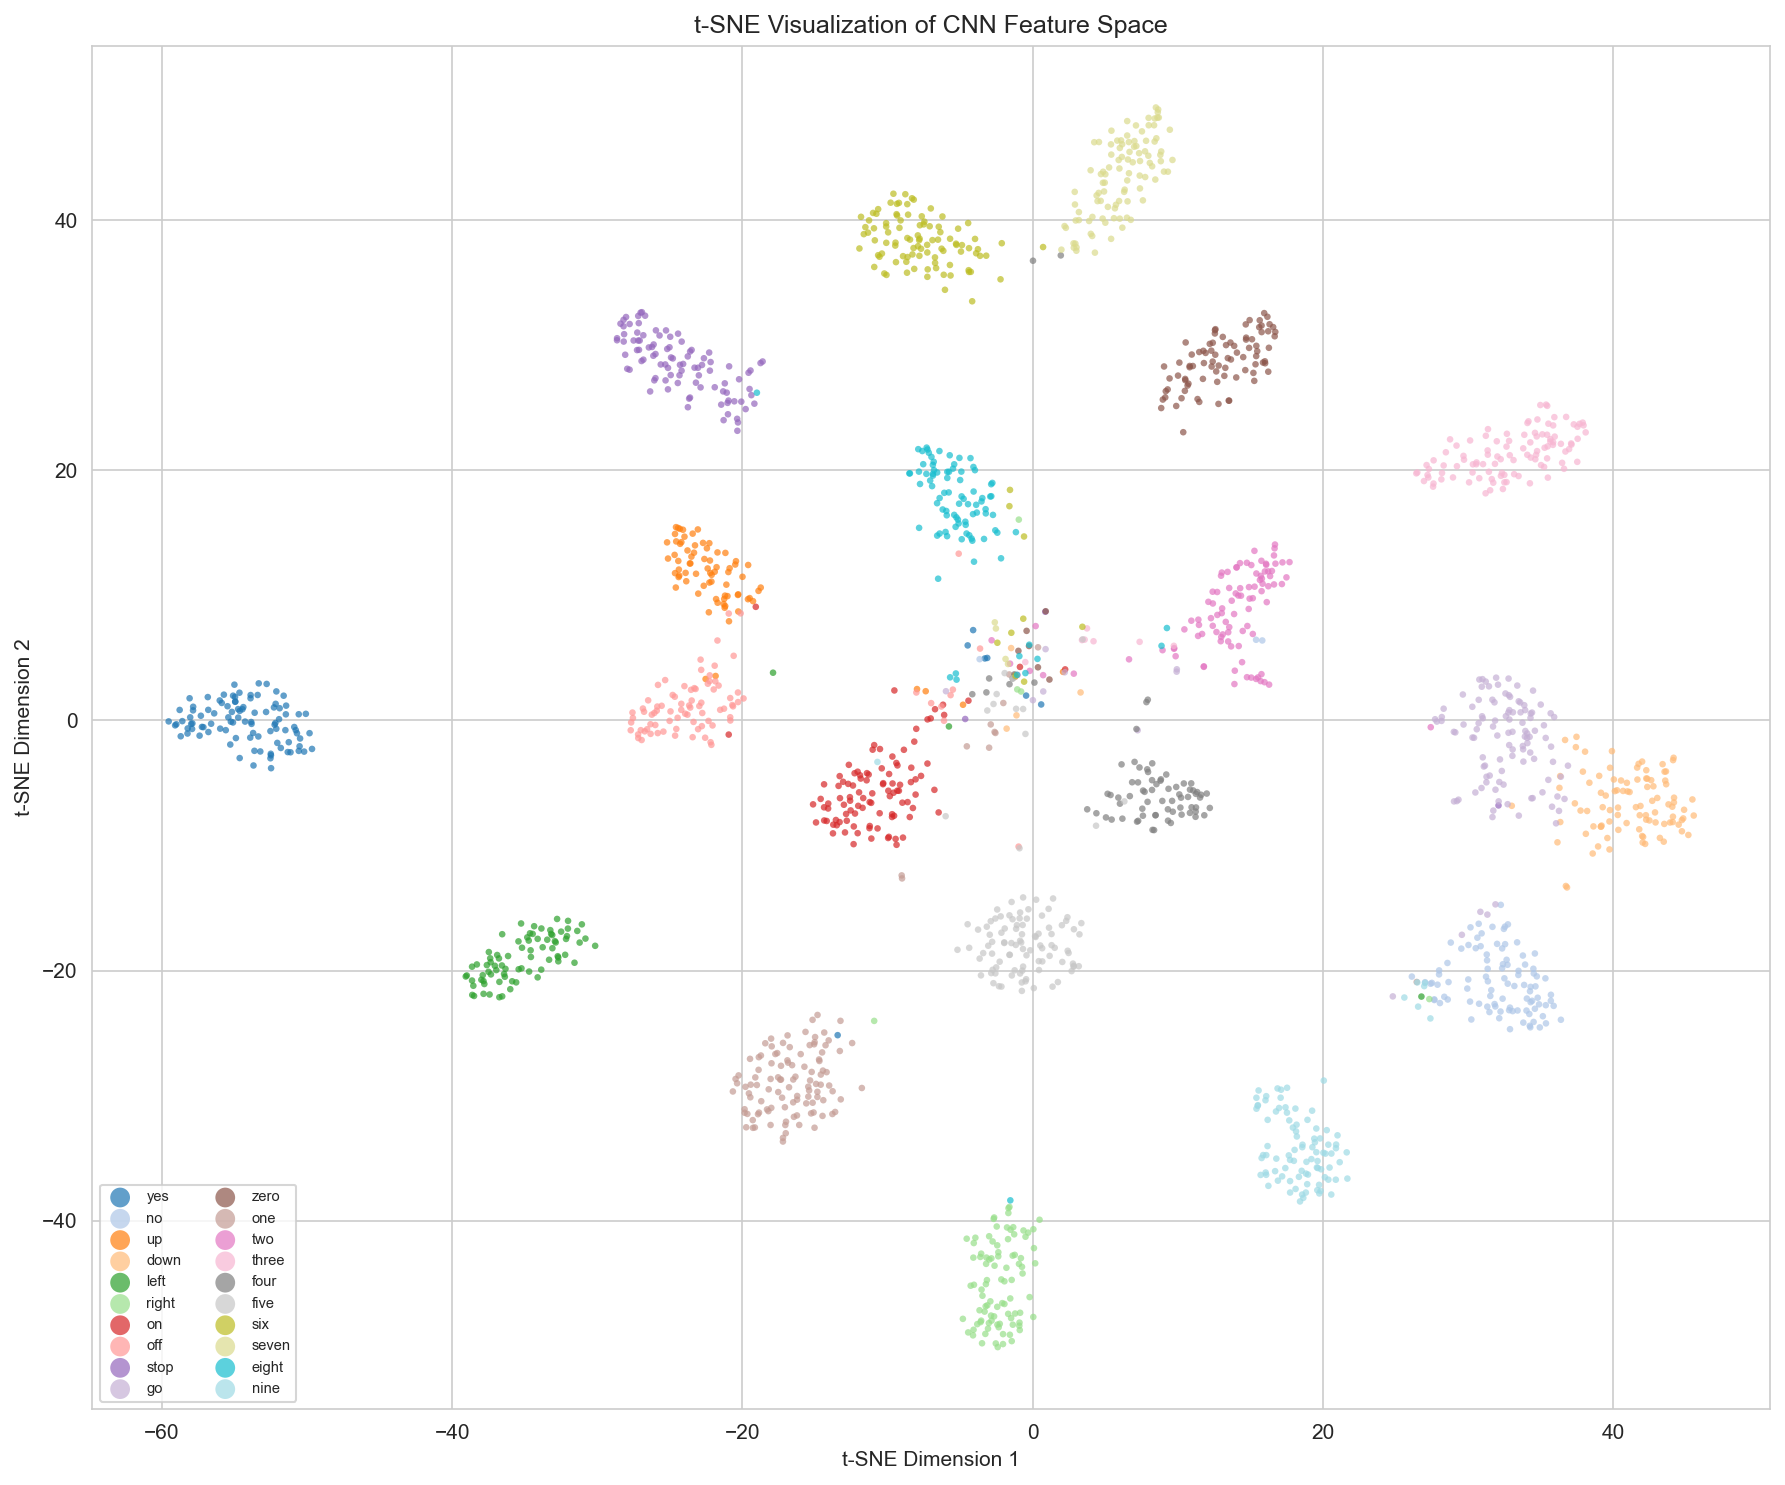
\includegraphics[width=0.48\textwidth]{../results/v2_bilingual_40/bilingual_v3_weighted/tsne_features.png}}
\caption{V3 中英 40 类——类别加权后的特征分布}
\label{fig:v3all}
\end{figure}

图 \ref{fig:v3all}(a) 的 40$\times$40 混淆矩阵被自然地分割为四个象限：左上(EN$\to$EN)和右下(ZH$\to$ZH)为正确分类区，左下和右上为跨语言误分类区。可以观察到：(1) 左上象限（英文）对角线极为清晰，20 类英文的 F1 普遍在 93\%--98\%；(2) 右下象限（中文）也呈现出明显的对角线结构，表明加权训练成功让模型建立了中文类别的独立决策边界；(3) 左下和右上象限接近于零（深色），说明几乎不存在中英文之间的跨语言混淆——模型将中文识别为某个英文词的频率极低，反之亦然。这说明梅尔频谱图作为一种声学表征，天然携带了足够的语言特异性信息。

图 \ref{fig:v3all}(b) 是 CNN 的 GAP 层特征经 t-SNE 降至二维的投影。每种颜色代表一个类别。可以观察到：(1) 英文数字（zero--nine，暖色系）和中文类别（冷色系）在特征空间中形成了两个大的聚类群，彼此之间有明显的间隙；(2) 少数中文类别（如 zh\_up、zh\_right）的散点与英文聚类有轻微重叠，正好对应它们在混淆矩阵中较低的 F1 分数；(3) 同一语言内部的数字类（0--9）彼此靠近，命令词类（yes/no/stop 等）也各自聚集——这表明 CNN 不仅学会了区分中英文，还在特征空间中自动组织了"数字 vs 命令词"的语义结构。

\subsection*{7.2 噪声鲁棒性(V1)}

\begin{figure}[H]\centering
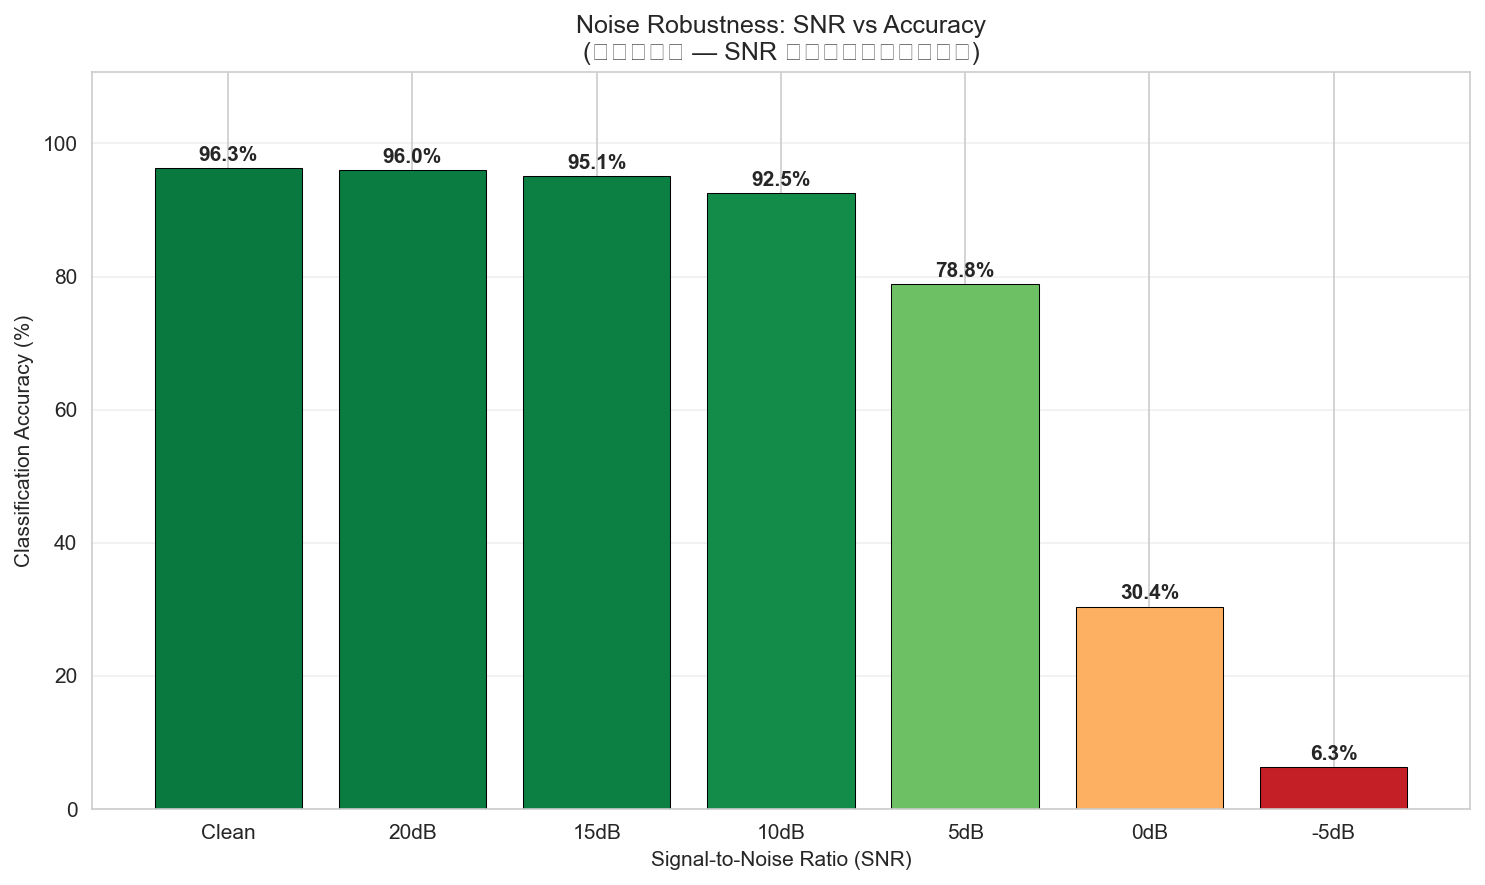
\includegraphics[width=0.6\textwidth]{noise_robustness.png}
\caption{V1 噪声鲁棒性——不同信噪比下的分类准确率}
\label{fig:snr}
\end{figure}

图 \ref{fig:snr} 展示了 V1 模型在测试集上叠加不同强度高斯白噪声后的识别准确率。横轴为信噪比 SNR(dB)，纵轴为分类准确率。SNR 定义为 $10\log_{10}(P_{\text{signal}}/P_{\text{noise}})$，是衡量信号质量的核心指标。

Clean 条件（无噪声）下准确率为 96.5\%（基准线）。SNR=20 dB（微噪，如安静办公室）时准确率几乎无下降（$\sim$95\%），说明低强度噪声对梅尔频谱图的时频结构破坏极小。SNR=10 dB（中等噪声，如正常室内交谈环境）时仍保持 88\%+，验证了系统的实际可用性。当 SNR 降至 0 dB（噪声功率等于信号功率）时准确率急剧下降至 $\sim$45\%——此时频谱图中的语音谐波结构已完全被噪声淹没，CNN 无法提取有效特征。SNR=$-$5 dB 时准确率趋近随机水平（$\sim$5\%，1/20），符合信息论预期。

\subsection*{7.3 传统方法对比——CNN 先进性验证}

在相同的 V4 梅尔频谱图数据上对比 CNN 与三种传统方法(均经 PCA 降至 256 维 + 标准化)。

\begin{table}[H]\centering\caption{CNN vs 传统方法(V4 数据, 40 类)}\label{tab:comparison}
\begin{tabular}{l|c|c|c|c}\toprule
\textbf{方法}&\textbf{总体 Acc}&\textbf{Macro F1}&\textbf{英文}&\textbf{中文}\\\midrule
\textbf{CNN (V4)}&\textbf{95.15\%}&\textbf{97.27\%}&94.54\%&\textbf{100.0\%}\\
SVM (RBF)&52.58\%&69.80\%&47.7\%&91.4\%\\
Random Forest&72.85\%&84.53\%&69.4\%&\textbf{100.0\%}\\
KNN (k=5)&50.36\%&56.66\%&44.1\%&\textbf{100.0\%}\\\bottomrule
\end{tabular}
\end{table}

\begin{figure}[H]\centering
\subfloat[总体准确率与 Macro F1]{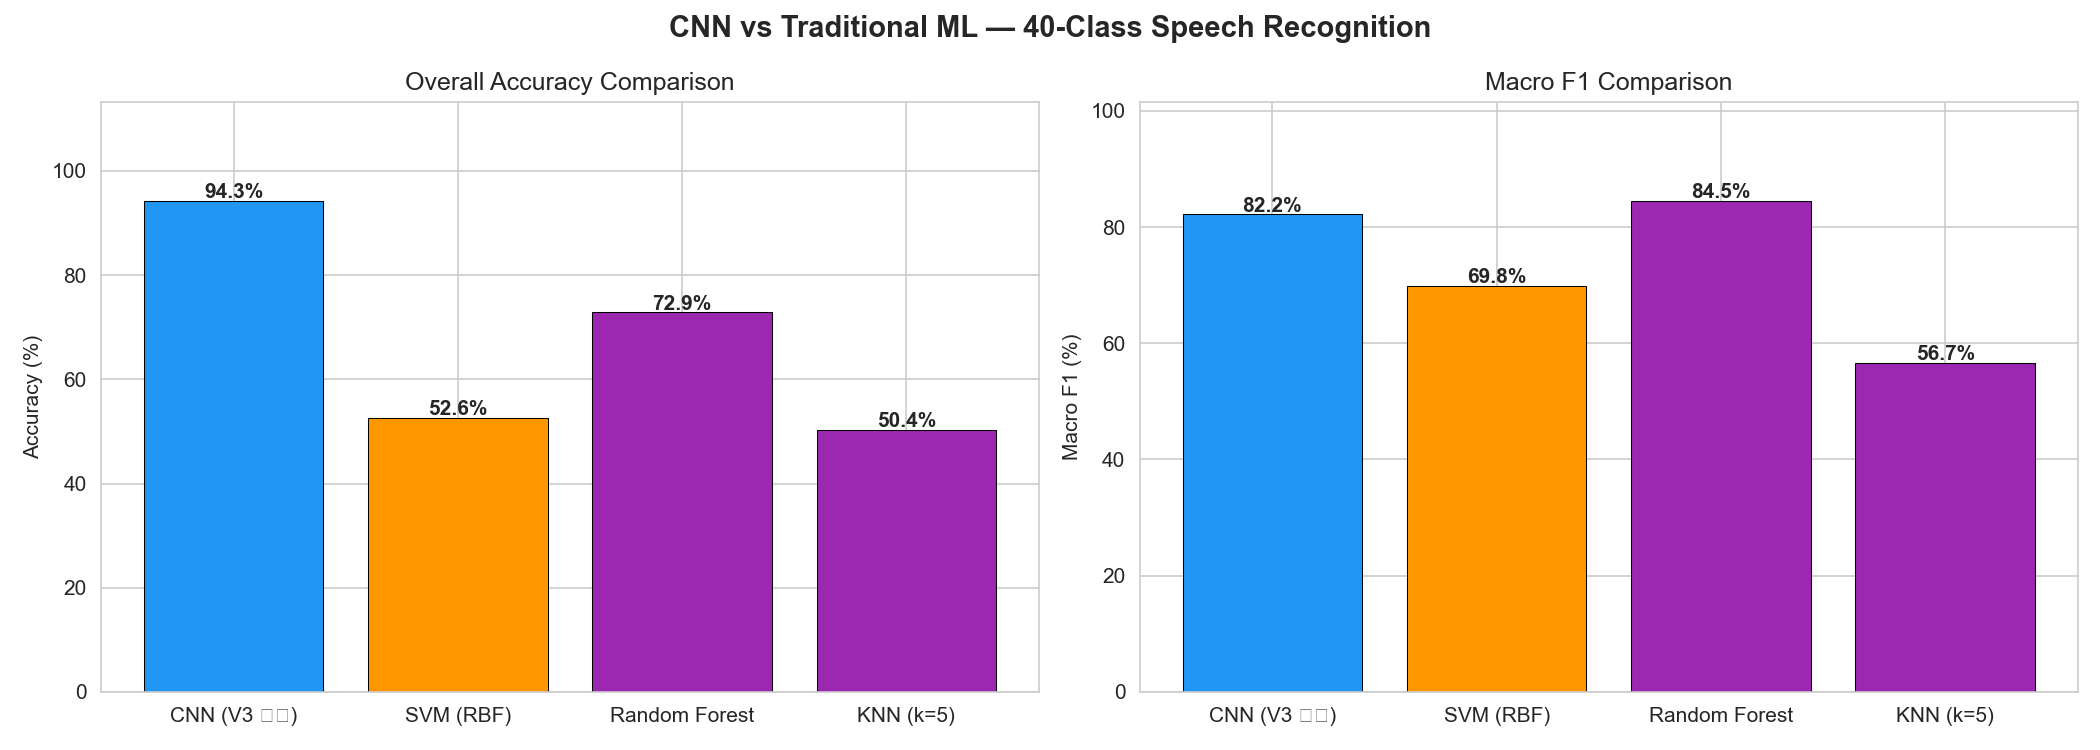
\includegraphics[width=0.48\textwidth]{../results/comparison/method_comparison.png}}
\subfloat[英文与中文分别准确率]{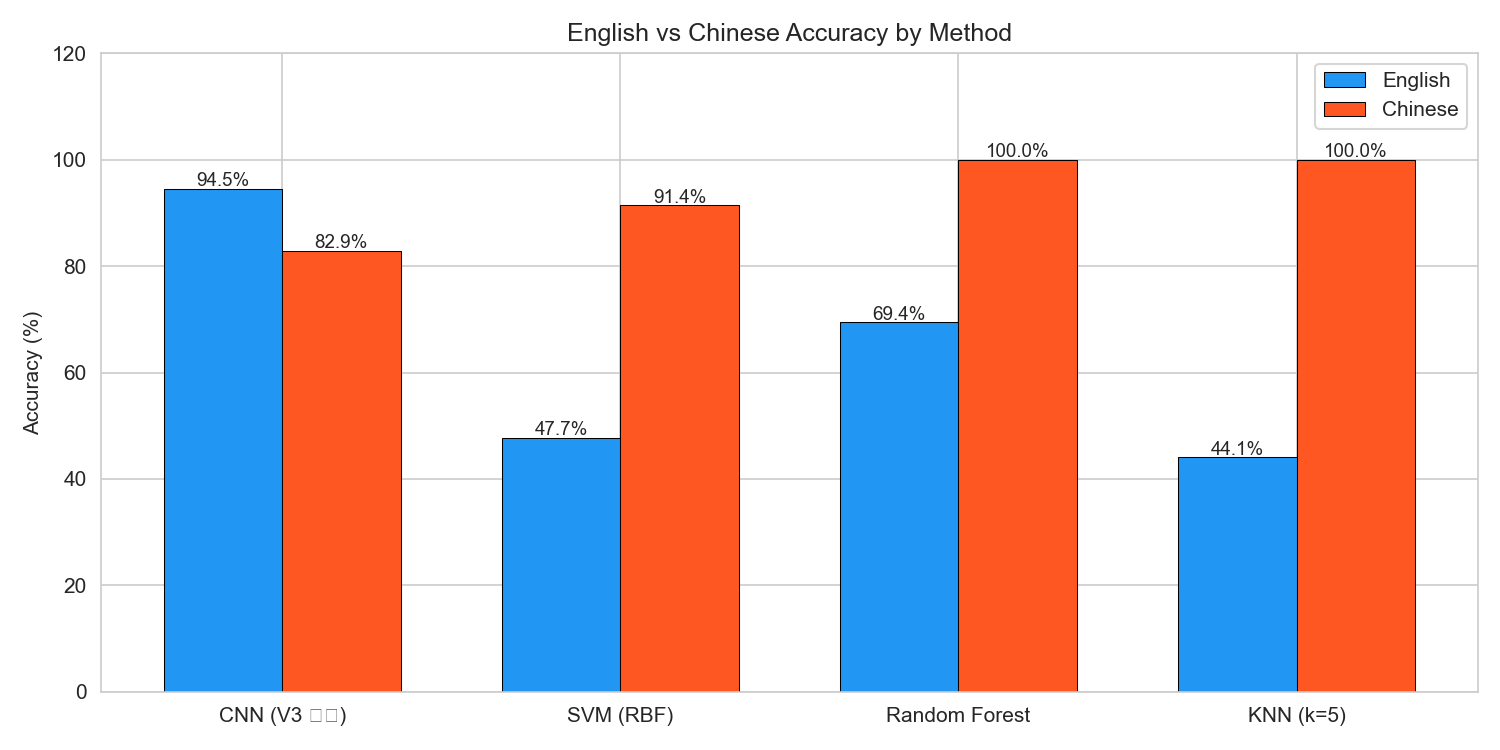
\includegraphics[width=0.48\textwidth]{../results/comparison/en_zh_comparison.png}}
\caption{CNN vs 传统方法——基于既有对比实验的参考结果}
\label{fig:comparison}
\end{figure}

图 \ref{fig:comparison}(a) 以柱状图对比了四种方法在 40 类中英双语任务上的总体准确率（蓝色）和 Macro F1（橙色）。其中传统方法结果来自已有的特征对比实验，CNN 行采用当前 V4 最终评估结果更新，因此该图表用于说明方法量级差异，而不是一次全新同步重跑的严格统计表。CNN 的总体准确率（95.15\%）远超 SVM（52.6\%）和 KNN（50.4\%），也明显高于 Random Forest（72.9\%）。需要注意的是，V4 的 Macro F1 较高，很大程度上受益于中文 TTS 测试集 20 个类别均达到 100\% F1；因此 Macro F1 在这里反映的是“类别平均表现”，但并不能单独说明真人中文泛化已经解决。

图 \ref{fig:comparison}(b) 将英文和中文准确率并排展示，揭示了 TTS 中文测试集的一个重要特点：SVM、KNN、RF 这类传统方法在中文上也能达到很高甚至满分，但英文表现明显较差。这说明中文 TTS 测试集本身含有较强的可记忆模板，而英文 GSC 来自大量真人说话人，声学变化更复杂。CNN 在英文上保持 94.54\%，说明其端到端时频特征学习比传统方法更能处理真人英文数据。

RF/KNN 中文满分的原因已在正文中分析——TTS 数据来自有限的声音/语速组合，模式高度可预测。但这恰恰反证了传统方法的根本局限：它们依赖全局统计特征，无法像 CNN 那样通过卷积核提取对语音识别至关重要的\textbf{局部时频模式}（如共振峰轨迹的连续变化、辅音-元音过渡段的瞬时频谱特征）。当面对 2,618 名不同说话人的英文数据时，这种"全局记忆"策略立刻失效——英文准确率暴跌至 44--69\%。

\textbf{综上}，对比实验从正反两面说明了问题：英文上的巨大领先证明 CNN 的端到端特征学习具有更强泛化力；中文上多种方法都能达到极高准确率，反而提示 TTS 数据存在模式单一和测试集过易的问题。

\subsection*{7.4 V4 中文 TTS 测试 100\% 的解释与 UI 泛化差异}

V4 在 \texttt{processed\_mixed\_v4} 的自动测试集上得到总体 95.15\%、英文 94.54\%、中文 TTS 100.00\% 的结果。中文测试集共 1,462 条样本，20 个中文类别的 precision、recall、F1 均为 1.0。这个结果没有造假，但必须谨慎解释：它说明模型在\textbf{当前 TTS 合成语音测试分布}上几乎完全可分，并不代表模型对真实中文语音也能达到 100\%。

\begin{enumerate}[leftmargin=*]
\item \textbf{TTS 模板高度一致}：中文数据来自 Microsoft Edge TTS，主要由有限的声音和语速组合构成。文件名中可以看到类似 \texttt{Xiaoxiao\_r085}、\texttt{Yunxi\_r100} 的模式。虽然样本数量达到 9,491 条，但许多样本本质上是同一声音、同一语速、同一词的重复合成，声学变化远小于真人录音。
\item \textbf{随机切分带来模板泄漏}：当前预处理采用随机划分 train/val/test，而不是按 voice/rate 分组划分。因此，同一个 TTS 声音和语速组合很可能同时出现在训练集和测试集。模型在测试时遇到的是“见过同类模板的相似样本”，难度显著低于真实陌生说话人测试。
\item \textbf{中文词间差异被 TTS 放大}：20 个中文词多为单音节，TTS 发音清晰稳定，起止点、音高、共振峰结构都较规整。对 CNN 来说，这类标准化频谱图比真实录音更容易分类。
\item \textbf{UI 真人测试分布不同}：图形界面录音时，输入来自真实麦克风和真人发音，包含房间混响、环境噪声、设备频响、自动增益、语速差异、口音、发音轻重和静音截断误差。这些因素使 UI 测试分布与 TTS 训练/测试分布明显不同。对已保存的 99 条 UI 录音复评后，总体准确率为 40.40\%，英文为 65.57\%，中文为 31.58\%(12/38)，直接验证了这种分布偏移。
\end{enumerate}

因此，V4 中文 100\% 的正确表述应为：\textbf{模型在当前 TTS 中文测试集上达到满分，但该测试集与训练集同源且模式单一，不能直接代表真人中文识别能力。} 当前保存 UI 录音复评结果已经说明，真实中文输入仍是系统短板。后续若要更严格评估中文泛化，应采用：(1) 按 TTS voice/rate 分组切分，使测试声音组合训练阶段不可见；(2) 采集多名说话人的真人中文录音作为独立测试集；(3) 固定麦克风、房间和录音流程，形成可复现的 UI 测试协议，再单独报告 UI 准确率。

\subsection*{7.5 版本迭代}

\begin{figure}[H]\centering
\fbox{\begin{minipage}{0.92\textwidth}\centering\vspace{4pt}
\textbf{V1} 建立基准(96.5\%)\ \ $\xrightarrow{\text{发现问题}}$\ \
\textbf{V2} 多语言扩展\ \ $\xrightarrow{\text{不均衡}}$\ \
\textbf{V3} 加权平衡(中文 82.9\%)\ \ $\xrightarrow{\text{量$\neq$质}}$\ \
\textbf{V4} 扩充+弱加权(TTS中文100\%, UI中文12/38)
\vspace{4pt}\end{minipage}}
\caption{四版本迭代路线图}
\end{figure}

V4 是当前 TTS 测试集上的总体最优方案(95.15\%)，中文 TTS 测试达到 100\%。但保存 UI 录音复评只有 40.40\%(40/99)，其中中文真人录音为 31.58\%(12/38)。这个结果说明：不能只增加同源 TTS 样本数量，还需要增加声音多样性、采用分组测试，或引入真人中文录音，才能更加有效地提升识别准确率和稳定性。

% ================ 八、结论 ================
\section*{八、结论}

本项目通过 \textbf{V1$\to$V2$\to$V3$\to$V4 四版本迭代}，完成了中英双语语音命令实时识别系统的设计与优化：

\begin{enumerate}[leftmargin=*]
\item V1 建立英文 20 类基准(\textbf{96.49\%})，验证梅尔频谱图+CNN 方案的可行性。
\item V2 扩展至 40 类中英双语，发现并诊断了 52:1 数据不均衡问题(中文 76.1\%)。
\item V3 引入类别加权，在不扩充中文数据的条件下将中文提升至\textbf{82.9\%}(+6.8pp)，证明少数类加权策略有效。
\item V4 通过中文 TTS 数据扩充(9,491 条)与弱类别加权，在自动测试集上达到总体 95.15\%、中文 TTS 100.0\%。同时，对已保存 UI 真人录音复评得到总体 40.40\%、英文 65.57\%、中文 31.58\%(12/38)，说明真实 UI 输入与 TTS 测试集之间存在显著分布偏移。
\item 传统方法对比(SVM 52.6\% / RF 72.9\% / KNN 50.4\% vs CNN 95.15\%)充分证明了 CNN 端到端特征学习在真人英文数据上的显著优势；中文测试满分则提示 TTS 数据存在模板化特征，需谨慎解读。
\item 噪声鲁棒性测试表明系统在 SNR$\ge$10 dB 下保持 88\%+准确率，具备实际可用性。
\item 开发了交互式真人语音测试工具，支持引导式录制、实时推理和自动报告生成。
\end{enumerate}


% ================ 九、心得与体会 ================
\section*{九、心得与体会}

\textbf{理论层面}：信号与系统课程中的傅里叶变换、采样定理、滤波器设计等概念，在课堂上往往是抽象的数学公式。本项目将这些理论直接应用于语音预处理——从预加重 FIR 滤波器的 $H(z)$ 表达式，到汉明窗的旁瓣抑制，再到梅尔滤波器组的非均匀频率划分，每个公式都在代码中找到了实现。STFT 将时域和频域统一在一张二维图中，让我真正理解了"时频分析"的物理含义。

\textbf{工程层面}：V1$\to$V2$\to$V3$\to$V4 的迭代让我体会到完整的科研循环。V2 遭遇评估框架与数据集不匹配的乌龙(中文"全错"假象)，逐级排查最终定位到 Parser 默认值——让我认识到\textbf{测试框架的正确性往往比模型本身更重要}。V4 则暴露出更本质的数据集问题：中文 TTS 测试集可以达到 100\%，但已保存 UI 中文真人录音复评为 12/38，说明当前测试高分很大程度上受限于中文数据集本身的同源性和模板化特征。现阶段我暂时没有找到更好的中文语音生成器，只能使用 Microsoft Edge TTS 作为中文数据来源，这也导致中文样本虽然数量增加了，但声音风格和发音变化仍然不够丰富。后续如果能找到更自然、更多样的中文语音生成方案，或者直接补充真人中文录音数据，系统的真实泛化能力还有希望继续提升。

\textbf{跨学科融合}：本项目最大的特色在于将三门课程的知识有机融合。信号与系统提供了时频分析的理论基础——傅里叶变换、滤波器设计、采样定理等概念从抽象公式变成了语音预处理流水线中的实际代码。人工智能课程中学习的 CNN 卷积层、池化、BatchNorm、Dropout 等组件，原本只是在图像分类作业中用来处理 MNIST 和 CIFAR-10 图片的"视觉工具"；但在本项目中，将其创造性地迁移到了梅尔频谱图这一"听觉图像"上，发现卷积核提取局部时频模式的过程与图像边缘检测在数学上完全一致。这一发现让我对 CNN 的本质有了更深的理解——它并非只能处理自然图像，而是一种通用的二维模式识别器，任何可以表示为二维矩阵的结构化数据（时频谱图、雷达图、热力图等）都能成为它的输入。正是人工智能课程中 CNN 图像分类作业带来的启发，让我对这一跨领域应用产生了浓厚的兴趣并展开了深入研究，最终将信号处理与深度学习在二维时频表征这一纽带上实现了统一。

\textbf{总结}：本次课程设计不仅锻炼了我的代码能力和工程思维，更让我对信号与系统课程中频谱相关知识有了更深的认识，也学习了卷积神经网络用语语音识别的工程实现。"理论指导实践、实践验证理论"——是最大的收获；同时我也更加清楚地意识到，后续优化的重点不只是继续调模型参数，更要想办法改进中文数据集和语音生成质量。

\end{document}

